\documentclass[xcolor=dvipsnames]{beamer}
\usepackage[utf8]{inputenc}
\usepackage[T1]{fontenc}
\usepackage{lmodern}
\usepackage{xcolor}
\usepackage{color}
\usepackage{enumitem}
\usepackage{tikz}
\usepackage{listings}

\setlist[itemize,1]{label=\textbullet}
\setlist[itemize,2]{label=$-$}

%\usebackgroundtemplate{\includegraphics[width=\paperwidth,height=\paperheight]{images/forma4.png}}
\setbeamercolor{frametitle}{bg=Gray, fg=white}
\setbeamercolor{normal text}{fg=black}

\setbeamercolor{title}{fg=white}
\setbeamercolor{titlelike}{fg=white}
\setbeamercolor{structure}{bg=Gray, fg=black}
\useoutertheme{shadow}
%\useinnertheme{rounded}

\beamertemplatenavigationsymbolsempty

\setbeamertemplate{footline}[frame number] 
\setbeamertemplate{headline}{}

%\renewcommand*{\bibfont}{\footnotesize}
\bibliographystyle{plain}

\renewcommand{\figurename}{Abb.}
\renewcommand{\tablename}{Tab.}
\lstset{aboveskip=20pt,belowskip=20pt,belowcaptionskip=20pt,abovecaptionskip=20pt}


\title{Optimierung und Übertragung von Tiefengeometrie
für Remote-Visualisierung}
\author{Josef Schulz}
\institute{Technische Universität Dresden}

\begin{document}

\begin{frame}
	\maketitle
	\nocite*{}
	\thispagestyle{empty}
\end{frame}

\section{Motivation}
\begin{frame}
	\frametitle{Motivation}
	\begin{figure}
	\centering
	\begin{tikzpicture}
	\node [
		label=below:Super Computer
	] (sc) at (0, 0) {
\includegraphics[width=2cm]{icons/supercomputer}};
	
	
	\node [
	    label=center:Internet,
	] (inet) at (3, 0) {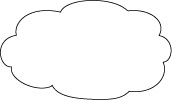
\includegraphics[width=3cm]{icons/cloud}};
	
	\node [
		label=below:Client	
	] (cl) at (6, 0) {
\includegraphics[width=2cm]{icons/pc}};
	
	\draw[->, bend right=45] (cl.north west) to (sc.north east);
	\draw[->, bend right=45] (sc.south east) to (cl.south west);
	\end{tikzpicture}
	
		\end{figure}
\end{frame}

\begin{frame}
	\frametitle{Aufgabenstellung}
	
	Grundlegendes:
	\begin{itemize}
		\item Entwicklung eines Remote-Visualisierungssystems
		\item Client basiert auf JavaScript, WebGl
		\item Kommunikation findet über WebSocket-Protokoll statt
	\end{itemize}
	\vspace{1cm}
	
	\begin{itemize}
		\item Approximation der entstehenden Tiefenbilder durch Dreiecksnetze
		\item Auswertung der Resultate in Abhängigkeit des Winkelunterschieds anhand von Ground-Truth-Szenen
	\end{itemize}
\end{frame}

\begin{frame}
	\frametitle{Herausforderungen}
	
	\vspace*{0.4cm}
	
	\begin{itemize}
		\setlength{\itemsep}{8pt}
		
		\item Anwendung der Approximation auf Partikelbasierte Datensätze
		\item 
	\end{itemize}
	
\end{frame}

\begin{frame}
	\frametitle{Gliederung}
	\tableofcontents
\end{frame}

\section{Verwandte Arbeiten}
\begin{frame}
\frametitle{Verwandte Arbeiten}

	\begin{itemize}
		\item THIN Systeme
		\item cluster
		\item 3D gaming ---
	\end{itemize}
\end{frame}

\section{Grundlagen}

\subsection{Szenen}

\begin{frame}
\frametitle{TestSpheres}
	\begin{columns}
		\begin{column}{5cm}
			\begin{figure}
				\includegraphics[width=\textwidth]{../Scenes/TestSpheres/run_1/testspheres_00000.png}
				\caption{Farbbild}
			\end{figure}
		\end{column}
		\begin{column}{5cm}
			\begin{figure}
				\includegraphics[width=\textwidth]{../Scenes/TestSpheres/run_1/testspheres_00000_depth.png}
				\caption{Tiefenbild}
			\end{figure}
		\end{column}
	\end{columns}
\end{frame}

\begin{frame}
\frametitle{CoolRandom}
	\begin{columns}
		\begin{column}{5cm}
			\begin{figure}
				\includegraphics[width=\textwidth]{../Scenes/CoolRandom/run_1/coolrandom_00000.png}
				\caption{Farbbild}
			\end{figure}
		\end{column}
		\begin{column}{5cm}
			\begin{figure}
				\includegraphics[width=\textwidth]{../Scenes/CoolRandom/run_1/coolrandom_00000_depth.png}
				\caption{Tiefenbild}
			\end{figure}
		\end{column}
	\end{columns}
\end{frame}

\begin{frame}
	\frametitle{Aufteilung}
	
	\begin{table}[h]
		\begin{tabular}{c|c|c|c|c}
			\# & Anzahl Bilder & min Winkel &  max Winkel & Winkel Schritt \\
			\hline
			1 & 241 & 0  & 5  & 0.25 \\
			2 & 60  & 6  & 10 & 1 	 \\
			3 & 192 & 15 & 90 & 5  	 \\
		\end{tabular}
		\centering
	\end{table}
	
\end{frame}

\subsection{Rückprojektion}
\begin{frame}
\frametitle{Rückprojektion einer Punktwolke}

\begin{figure}
	\begin{tikzpicture}
		\node[inner sep=0pt] (depth) at (0,0)
		    {\includegraphics[width=.25\textwidth]{../Scenes/TestSpheres/run_1/testspheres_00000_depth.png}};
		
		\node[] (model) at (8, -2) {\includegraphics[width=.25\textwidth]{images/PointExamples.png}};
		
		\node[inner sep=0pt] (result) at (0,-4)
	    {\includegraphics[width=.25\textwidth]{../Scenes/TestSpheres/run_3/testspheres_00015_depth.png}};
	    
	    \draw[->] (depth) to node[auto] {$v' = (P \cdot V \cdot M)^{-1} \cdot v$} (model);
	    \draw[->] (model) to node[auto] {$v'' = (P_i \cdot V_i \cdot M_i) \cdot v' $} (result);
	\end{tikzpicture}
	
\end{figure}

\end{frame}

\section{Methoden}

\begin{frame}
	\frametitle{Gradientenbilder}
	
	Die Gradientenbilder, wurden mit dem Sobel-Operator erzeugt:
	
	\begin{columns}
		\begin{column}{5cm}
			\begin{figure}
				\includegraphics[width=\textwidth]{../results/7/512x512_Delaunay/D10/L0.0/I0.0/_pre/gx.png}
				\caption{$\mid \nabla_x \mid$}
			\end{figure}
		\end{column}
		\begin{column}{5cm}
			\begin{figure}
				\includegraphics[width=\textwidth]{../results/7/512x512_Delaunay/D10/L0.0/I0.0/_pre/gy.png}
				\caption{$\mid \nabla_y \mid$}
			\end{figure}
		\end{column}
	\end{columns}
\end{frame}

\begin{frame}
	\frametitle{Quadtree-Ansatz}
	\begin{figure}
		\centering
		\begin{tikzpicture}
			\draw (0,0) -- (8,0) -- (8,6) -- (0,6) -- cycle;
			\draw (4,0) -- (4,6);
			\draw (0,3) -- (8,3);
			\node at (2, 4.5) {$R_1$};
			\node at (6, 4.5) {$R_2$};
			\node at (2, 1.5) {$R_3$};
			\node at (6, 1.5) {$R_4$};
			\node[circle, minimum width=1em,fill=OliveGreen] at (4,0) {};
			\node[circle, minimum width=1em,fill=OliveGreen] at (8,3) {};
			\node[circle, minimum width=1em,fill=OliveGreen] at (0,3) {};
			\node[circle, minimum width=1em,fill=OliveGreen] at (4,6) {};
			\node[circle, minimum width=1em,fill=OliveGreen] at (4,3) {};
		\end{tikzpicture}
	\end{figure}
\end{frame}

\begin{frame}
	\frametitle{Quadtree: Finden der Seed-Points}

	\begin{align}
	c_x &= \max\limits_{R} \mid \nabla_x \mid - \min\limits_{R} \mid \nabla_x \mid \\
	c_y &= \max\limits_{R} \mid \nabla_y \mid - \min\limits_{R} \mid \nabla_y \mid
	\end{align}
	
	Punkte die zum Hintergrund gehören werden verworfen.
\end{frame}

\begin{frame}

	\begin{tikzpicture}
		\node[] (s) at (0, 0) {\includegraphics[width=.4\textwidth]{../results/7/512x512_Delaunay/D10/L0.6/I0.4/_pre/seeds.png}};
		
		\node[] (d) at (7, 0) {\includegraphics[width=.4\textwidth]{../results/7/512x512_Delaunay/D10/L0.6/I0.4/_pre/delaunay.png}};
		
		\draw[->] (s) to node[auto] {delaunay} (d);
	\end{tikzpicture}
\end{frame}

\begin{frame}
	\frametitle{Floyed Steinberg-Ansatz}
	
	Erzeugung einer Feature-Map aus den Gradientenbildern:
	\begin{equation}
		\sigma_p = \left( \frac{\parallel \nabla p \parallel}{A} \right)^\gamma.
		\label{eq:featureMap}
	\end{equation}
	
\end{frame}

\begin{frame}[fragile]
	\frametitle{test}
	\begin{tiny}
	
	\begin{lstlisting}[numbers=left,
					   mathescape=true,
					   xleftmargin=0.1\textwidth,
					   captionpos=b,
					   caption={Floyd-Steinberg-Algorithmus}]
	for each y
		for each x
		   oldpixel        := pixel[x][y]
		   newpixel        := (pixel[x][y] > $\delta$) ? $\delta$ : 0
		   pixel[x][y]     := newpixel
		   quant_error     := oldpixel - newpixel
		   pixel[x+1][y  ] := pixel[x+1][y  ] + quant_error * 7 / 16
		   pixel[x-1][y+1] := pixel[x-1][y+1] + quant_error * 3 / 16
		   pixel[x  ][y+1] := pixel[x  ][y+1] + quant_error * 5 / 16
		   pixel[x+1][y+1] := pixel[x+1][y+1] + quant_error * 1 / 16
	\end{lstlisting}
	
	\end{tiny}
\end{frame}

\begin{frame}
		
	\begin{tikzpicture}
		\node[] (s) at (0, 0) {\includegraphics[width=.4\textwidth]{../results/7/512x512_Delaunay/T0.5/G0.6/featuremap.png}};
		
		\node[] (d) at (7, 0) {\includegraphics[width=.5\textwidth]{../results/7/512x512_Delaunay/T0.5/G0.6/delaunay.png}};
		
		\draw[->] (s) to node[auto] {delaunay} (d);
	\end{tikzpicture}
\end{frame}

\begin{frame}
	\frametitle{Netzoptimierung}
	
	\begin{itemize}
		\item Wann ist eine Kante nicht valid
		\item Wann muss ein Dreieck nachbearbeitet werden.
	\end{itemize}
\end{frame}

\begin{frame}
	\frametitle{Valide Kanten}
	
	$p_1, p_2$ - Eckpunkte der Kante \\
	$p_{m}$	- Mittelpunkt auf der Kante \\
	
	\vspace{.5cm}
	
	Ist eine der folgenden Bedingungen nicht erfüllt wird die Kante 
	als nicht valid bezeichnet:
	
	\begin{equation}
		\frac{d_{p_1} + d_{p_2}}{2} - d_{p_m} < \varepsilon
	\end{equation}
		
	\begin{equation}
	\frac{\mid d_{p_1} - d_{p_2} \mid}{\parallel p_1 - p_2 \parallel (d_{p_1} + d_{p_2})} < \alpha
	\label{eq:EDGE_VALID}
	\end{equation}
	
\end{frame}

\begin{frame}
	Enthält ein Dreieck zwei nicht valide Kanten, ist das Dreieck nicht valide und
	wird nachbearbeitet:
	
	\begin{columns}
		\begin{column}{5cm}
			\begin{figure}
			
			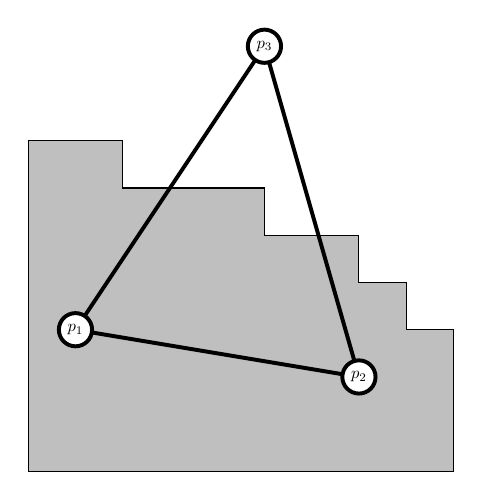
\begin{tikzpicture}[scale=0.6, every node/.style={scale=0.6}]
				\draw[fill=gray!50] (0, -5) -- (0, 2) -- (2, 2) -- (2, 1) -- (5, 1) -- (5, 0) --(7, 0) -- (7, -1) -- (8, -1) -- (8, -2) -- (9, -2) -- (9, -5) -- cycle;
				
				\begin{scope}[
					auto, vertex/.style={align=center, draw, fill=white, circle, line width=0.5mm, minimum width=2em, inner sep=2pt}]
					\node[vertex] (V1) at (1, -2) {$p_1$};
					\node[vertex] (V2) at (7, -3) {$p_2$};
					\node[vertex] (V3) at (5, 4) {$p_3$};
				\end{scope}
				
				\draw[-, line width=0.5mm] (V1) edge (V2);
				\draw[-, line width=0.5mm] (V2) edge (V3);
				\draw[-, line width=0.5mm] (V1) edge (V3);
			\end{tikzpicture}
			\caption{2 Kanten sind nicht valide}
			\end{figure}
		\end{column}
		\begin{column}{5cm}
			\begin{figure}
			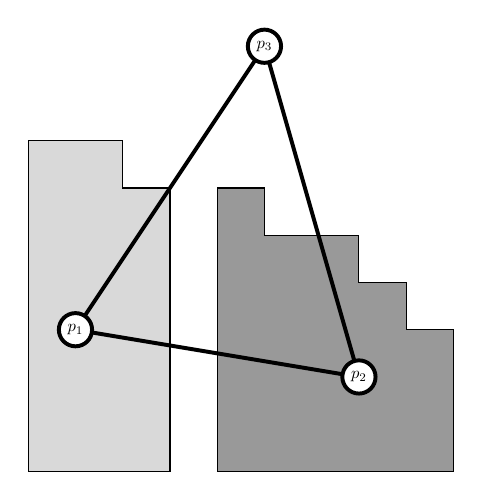
\begin{tikzpicture}[scale=0.6, every node/.style={scale=0.6}]
				\draw[fill=gray!30] (0, -5) -- (0, 2) -- (2, 2) -- (2, 1) -- (3, 1) -- (3, -5) -- cycle;
				
				\draw[fill=gray!80] (4, -5) -- (4, 1) -- (5, 1) -- (5, 0) -- (7, 0) -- (7, -1) -- (8, -1) -- (8, -2) -- (9, -2) -- (9, -5) -- cycle;
				
				\begin{scope}[
					auto, vertex/.style={align=center, draw, fill=white, circle, line width=0.5mm, minimum width=2em, inner sep=2pt}]
					\node[vertex] (V1) at (1, -2) {$p_1$};
					\node[vertex] (V2) at (7, -3) {$p_2$};
					\node[vertex] (V3) at (5, 4) {$p_3$};
				\end{scope}
			
				\draw[-, line width=0.5mm] (V1) edge (V2);
				\draw[-, line width=0.5mm] (V2) edge (V3);
				\draw[-, line width=0.5mm] (V1) edge (V3);	
			\end{tikzpicture}
			\caption{2 Kanten sind nicht valide}
			\end{figure}
		\end{column}
	\end{columns}
\end{frame}

\begin{frame}
	\frametitle{2 Kanten sind nicht Valide}

	\begin{columns}
		\begin{column}{5cm}
				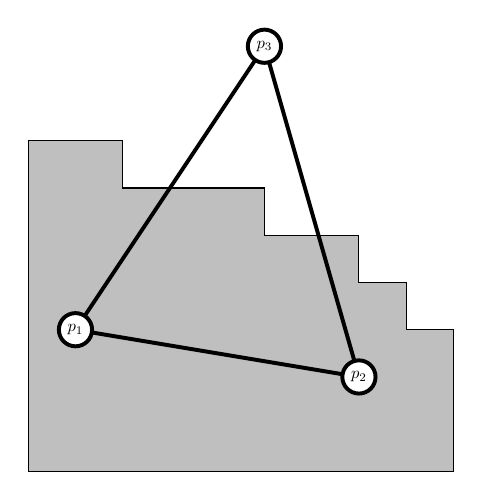
\begin{tikzpicture}[scale=0.6, every node/.style={scale=0.6}]
					\draw[fill=gray!50] (0, -5) -- (0, 2) -- (2, 2) -- (2, 1) -- (5, 1) -- (5, 0) --(7, 0) -- (7, -1) -- (8, -1) -- (8, -2) -- (9, -2) -- (9, -5) -- cycle;
					
					\begin{scope}[
						auto, vertex/.style={align=center, draw, fill=white, circle, line width=0.5mm, minimum width=2em, inner sep=2pt}]
						\node[vertex] (V1) at (1, -2) {$p_1$};
						\node[vertex] (V2) at (7, -3) {$p_2$};
						\node[vertex] (V3) at (5, 4) {$p_3$};
					\end{scope}
					
					\draw[-, line width=0.5mm] (V1) edge (V2);
					\draw[-, line width=0.5mm] (V2) edge (V3);
					\draw[-, line width=0.5mm] (V1) edge (V3);
				\end{tikzpicture}
		\end{column}
		\begin{column}{5cm}
				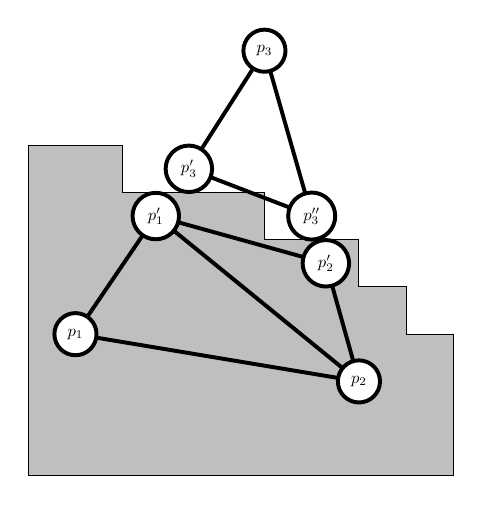
\begin{tikzpicture}[scale=0.6, every node/.style={scale=0.6}]
					\draw[fill=gray!50] (0, -5) -- (0, 2) -- (2, 2) -- (2, 1) -- (5, 1) -- (5, 0) --(7, 0) -- (7, -1) -- (8, -1) -- (8, -2) -- (9, -2) -- (9, -5) -- cycle;
					
					\begin{scope}[
						auto, vertex/.style={align=center, draw, fill=white, circle, line width=0.5mm, minimum width=2em, inner sep=5pt}]
						\node[vertex] (V1) at (1, -2) {$p_1$};
						\node[vertex] (V2) at (7, -3) {$p_2$};
						
						\node[vertex] (V13) at (2.7, 0.5) {$p_1'$};
						\node[vertex] (V23) at (6.3, -0.5) {$p_2'$};
						
						\node[vertex] (V3) at (5, 4) {$p_3$};
						
						\node[vertex] (V31) at (3.4, 1.5) {$p_3'$};
						\node[vertex] (V32) at (6, 0.5) {$p_3''$};
					\end{scope}
					
					\draw[-, line width=0.5mm] (V1) edge (V2);
					\draw[-, line width=0.5mm] (V1) edge (V13);
					\draw[-, line width=0.5mm] (V2) edge (V23);
					
					\draw[-, line width=0.5mm] (V13) edge (V23);
					\draw[-, line width=0.5mm] (V13) edge (V2);
					
					\draw[-, line width=0.5mm] (V3) edge (V31);
					\draw[-, line width=0.5mm] (V3) edge (V32);
					\draw[-, line width=0.5mm] (V31) edge (V32);
				\end{tikzpicture}
		\end{column}
	\end{columns}
\end{frame}

\begin{frame}
	\frametitle{3 Kanten sind nicht Valide}
	
	\begin{columns}
		\begin{column}{5cm}
		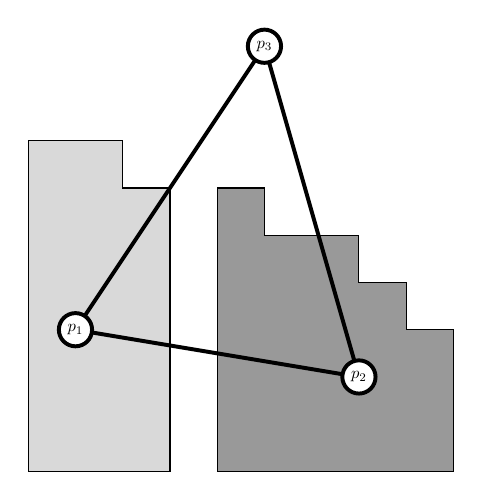
\begin{tikzpicture}[scale=0.6, every node/.style={scale=0.6}]
			\draw[fill=gray!30] (0, -5) -- (0, 2) -- (2, 2) -- (2, 1) -- (3, 1) -- (3, -5) -- cycle;
			
			\draw[fill=gray!80] (4, -5) -- (4, 1) -- (5, 1) -- (5, 0) -- (7, 0) -- (7, -1) -- (8, -1) -- (8, -2) -- (9, -2) -- (9, -5) -- cycle;
			
			\begin{scope}[
				auto, vertex/.style={align=center, draw, fill=white, circle, line width=0.5mm, minimum width=2em, inner sep=2pt}]
				\node[vertex] (V1) at (1, -2) {$p_1$};
				\node[vertex] (V2) at (7, -3) {$p_2$};
				\node[vertex] (V3) at (5, 4) {$p_3$};
			\end{scope}
		
			\draw[-, line width=0.5mm] (V1) edge (V2);
			\draw[-, line width=0.5mm] (V2) edge (V3);
			\draw[-, line width=0.5mm] (V1) edge (V3);	
		\end{tikzpicture}
		\end{column}
		\begin{column}{5cm}
		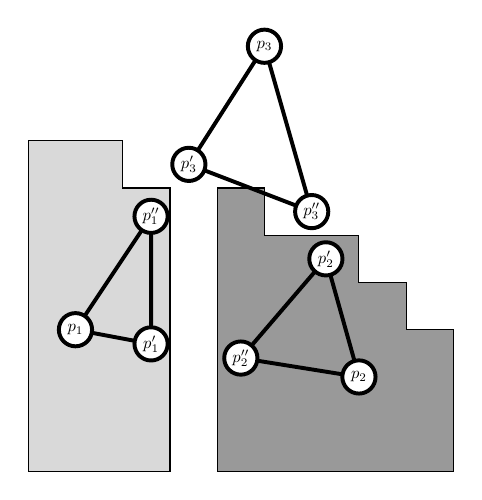
\begin{tikzpicture}[scale=0.6, every node/.style={scale=0.6}]
			\draw[fill=gray!30] (0, -5) -- (0, 2) -- (2, 2) -- (2, 1) -- (3, 1) -- (3, -5) -- cycle;
			
			\draw[fill=gray!80] (4, -5) -- (4, 1) -- (5, 1) -- (5, 0) -- (7, 0) -- (7, -1) -- (8, -1) -- (8, -2) -- (9, -2) -- (9, -5) -- cycle;
			
			\begin{scope}[
				auto, vertex/.style={align=center, draw, fill=white, circle, line width=0.5mm, minimum width=2em, inner sep=2pt}]
				\node[vertex] (V1) at (1, -2) {$p_1$};
				\node[vertex] (V2) at (7, -3) {$p_2$};
				
				\node[vertex] (V13) at (2.6, 0.4) {$p_1''$};
				\node[vertex] (V12) at (2.6, -2.3) {$p_1'$};
				
				\node[vertex] (V23) at (6.3, -0.5) {$p_2'$};
				\node[vertex] (V21) at (4.5, -2.6) {$p_2''$};
				
				\node[vertex] (V3) at (5, 4) {$p_3$};
				
				\node[vertex] (V31) at (3.4, 1.5) {$p_3'$};
				\node[vertex] (V32) at (6, 0.5) {$p_3''$};
			\end{scope}
			
			\draw[-, line width=0.5mm] (V1) edge (V12);
			\draw[-, line width=0.5mm] (V1) edge (V13);
			\draw[-, line width=0.5mm] (V12) edge (V13);
			\draw[-, line width=0.5mm] (V2) edge (V23);
			\draw[-, line width=0.5mm] (V2) edge (V21);
			\draw[-, line width=0.5mm] (V21) edge (V23);
			
			\draw[-, line width=0.5mm] (V3) edge (V31);
			\draw[-, line width=0.5mm] (V3) edge (V32);
			\draw[-, line width=0.5mm] (V31) edge (V32);
		\end{tikzpicture}
		\end{column}
	\end{columns}
\end{frame}

\section{Ergebnisse}
\begin{frame}
	\frametitle{JPEG PSNR}
	\begin{columns}
		\begin{column}{3cm}
			\begin{figure}
				\includegraphics[width=\textwidth]{images/jpeg_6_0.png}
				\caption{20,09 dB}
			\end{figure}
			\begin{figure}
				\includegraphics[width=\textwidth]{images/jpeg_6_60.png}
				\caption{25,24 dB}
			\end{figure}
		\end{column}
		\begin{column}{3cm}
			\begin{figure}
				\includegraphics[width=\textwidth]{images/jpeg_6_20.png}
				\caption{23,42 dB}
			\end{figure}
			\begin{figure}
				\includegraphics[width=\textwidth]{images/jpeg_6_80.png}
				\caption{27,07 dB}
			\end{figure}
		\end{column}
		\begin{column}{3cm}
			\begin{figure}
				\includegraphics[width=\textwidth]{images/jpeg_6_40.png}
				\caption{24,32 dB}
			\end{figure}
			\begin{figure}
				\includegraphics[width=\textwidth]{images/jpeg_6_100.png}
				\caption{28,05 dB}
			\end{figure}
		\end{column}
	\end{columns}
\end{frame}

\begin{frame}
	\frametitle{JPEG PSNR}
	\begin{columns}
		\begin{column}{3cm}
			\begin{figure}
				\includegraphics[width=\textwidth]{images/jpeg_7_0.png}
				\caption{27,25 dB}
			\end{figure}
			\begin{figure}
				\includegraphics[width=\textwidth]{images/jpeg_7_60.png}
				\caption{37,57 dB}
			\end{figure}
		\end{column}
		\begin{column}{3cm}
			\begin{figure}
				\includegraphics[width=\textwidth]{images/jpeg_7_20.png}
				\caption{34,88 dB}
			\end{figure}
			\begin{figure}
				\includegraphics[width=\textwidth]{images/jpeg_7_80.png}
				\caption{39,05 dB}
			\end{figure}
		\end{column}
		\begin{column}{3cm}
			\begin{figure}
				\includegraphics[width=\textwidth]{images/jpeg_7_40.png}
				\caption{36,63 dB}
			\end{figure}
			\begin{figure}
				\includegraphics[width=\textwidth]{images/jpeg_7_100.png}
				\caption{41,67 dB}
			\end{figure}
		\end{column}
	\end{columns}
\end{frame}

\section{Diskussion und Fazit}
\section{Fragen}

{\tiny\bibliography{literatur}}

\end{document}
